\documentclass[conference]{IEEEtran}
\usepackage{amsmath,amssymb,amsthm}
\usepackage{booktabs}
\usepackage{cite}
\usepackage{graphicx}
\usepackage{microtype}
\usepackage{subfig}
\usepackage{tikz}
\usetikzlibrary{arrows.meta,positioning,fit,calc}
\usepackage[hidelinks]{hyperref}
\usepackage{url}

\hypersetup{
  pdftitle={Native Binary-Weight Training Mitigates Post-Training Quantization Collapse in MNIST Diffusion},
  pdfauthor={Ayushman Bhattacharya, Anwesha Chakraborty, and Nihal Gazi},
  pdfkeywords={binary neural networks, diffusion models, quantization-aware training, post-training quantization, MNIST}
}

\newcommand{\dfid}{\ensuremath{\mathrm{dFID}}}
\newcommand{\dkid}{\ensuremath{\mathrm{dKID}}}
\newtheorem{proposition}{Proposition}

\begin{document}

\title{Native Binary-Weight Training Mitigates\\
Post-Training Quantization Collapse in MNIST Diffusion}

\author{
\IEEEauthorblockN{Ayushman Bhattacharya}
\IEEEauthorblockA{Pollinations AI\\ayushman.elixpo@gmail.com}
\and
\IEEEauthorblockN{Anwesha Chakraborty}
\IEEEauthorblockA{Dept. of CSE, JIS University\\anwesha.elixpo@gmail.com}
\and
\IEEEauthorblockN{Nihal Gazi}
\IEEEauthorblockA{Dept. of CSE (AI \& ML), IEM\\nihalg2006@gmail.com}
}

\maketitle

\begin{abstract}
Does failure after projecting a diffusion model to one-bit weights show that its
binary representation is unusable? We test that implication, rather than propose
a new quantizer, in a parameter-compatible MNIST residual U-Net. We compare
floating-point training, zero-shot one-bit-weight post-training quantization
(PTQ), binary-weight training from random initialization, floating-point
warm-started quantization-aware training (QAT), and a binary-weight/
binary-activation core. Every condition uses the same topology, data, optimizer,
per-stage budget, and 1,000-step ancestral sampler, with three independent
training seeds. Native W1A32 training obtains domain-feature Fr\'echet distance
$46.33\mathbin{\pm}17.24$, 28.4-fold lower than matched zero-shot PTQ
($1314.20\mathbin{\pm}314.96$), but remains substantially worse than FP32
($3.15\mathbin{\pm}0.38$). Warm QAT also recovers much of the PTQ loss, while
the W1A1 core retains a large distributional gap. A simple constrained-
optimization proposition formalizes why one projected floating-point optimum is
not an impossibility certificate for the binary hypothesis class. The supported
claim is deliberately local: on MNIST, training path explains a substantial
part of one-bit-weight PTQ collapse; this does not establish full W1A1 success,
floating-point parity, or transfer to natural images.
\end{abstract}

\begin{IEEEkeywords}
binary neural networks, diffusion models, post-training quantization,
quantization-aware training, MNIST
\end{IEEEkeywords}

\section{Introduction}

Diffusion models repeatedly evaluate a time-conditioned denoiser, making model
memory and arithmetic attractive compression targets. Binary neural networks
replace many real-valued weights by signs and optional scales
\cite{hubara2016bnn,rastegari2016xnornet}. At the extreme, BiDM studies binary
weights and activations (W1A1) and motivates specialized architecture and
distillation by the severe degradation of naive full binarization
\cite{bidm2024}. BinaryDM studies accurate weight binarization at W1A4
\cite{binarydm2025}.

A narrower logical question precedes those system designs: if a trained FP32
denoiser collapses after sign projection, has the binary-weight representation
failed, or has a point optimized for a different forward model simply been
projected poorly? Zero-shot PTQ evaluates only the projected FP32 solution.
BinaryConnect-style training instead maintains latent real parameters while
using binary weights in every forward pass\cite{courbariaux2015binaryconnect}.
The two procedures need not reach the same binary point.

We isolate this distinction on MNIST. All precision conditions share parameter
names, shapes, topology, optimizer, sampling procedure, and evaluation. The
experiment supports three findings:
\begin{itemize}
  \item native W1A32 training reduces \dfid{} by 28.4-fold relative to matched
  zero-shot PTQ, so PTQ collapse is not a certificate of binary-weight
  representational failure in this setting;
  \item warm-started QAT also recovers substantially, showing that random
  initialization is not uniquely necessary once binary forwards are optimized;
  and
  \item FP32 remains much better, while a W1A1 core remains weak; the result
  therefore neither contradicts the difficulty identified by BiDM nor
  establishes a general binary-diffusion solution.
\end{itemize}

The contribution is a controlled empirical distinction between projection and
optimization. The sign/scale quantizer, straight-through estimator (STE), and
residual components are standard and are not claimed as algorithmic novelty.

\section{Why PTQ Failure Is Not an Impossibility Result}

Let $\Theta_F$ be a floating-point parameter space, $\Theta_B$ the feasible
binary-weight space, $\mathcal L$ the diffusion training objective, and
$P:\Theta_F\rightarrow\Theta_B$ the sign/scale projection used by PTQ. Let
$\theta_F^\star$ minimize $\mathcal L$ over $\Theta_F$ and
$\theta_B^\star$ minimize it over $\Theta_B$.

\begin{proposition}[Projection non-implication]
The loss of a projected floating-point optimum is an upper bound on the optimal
binary-constrained loss:
\begin{equation}
\mathcal L(\theta_B^\star)
\leq \mathcal L(P(\theta_F^\star)).
\end{equation}
Consequently, poor performance of $P(\theta_F^\star)$ alone cannot establish
that every member of $\Theta_B$ performs poorly.
\end{proposition}

\begin{proof}
Because $P(\theta_F^\star)\in\Theta_B$, it is one feasible point in the
minimization defining $\theta_B^\star$. The minimum over $\Theta_B$ cannot have
higher loss than that particular feasible point.
\end{proof}

This elementary statement is not a convergence result. Native STE training is
not guaranteed to find $\theta_B^\star$, and diffusion quality is not determined
by training loss alone. It identifies exactly what the experiment must test:
whether optimization under binary forwards reaches a materially better feasible
point than zero-shot projection.

\begin{figure*}[t]
\centering
\resizebox{\textwidth}{!}{%
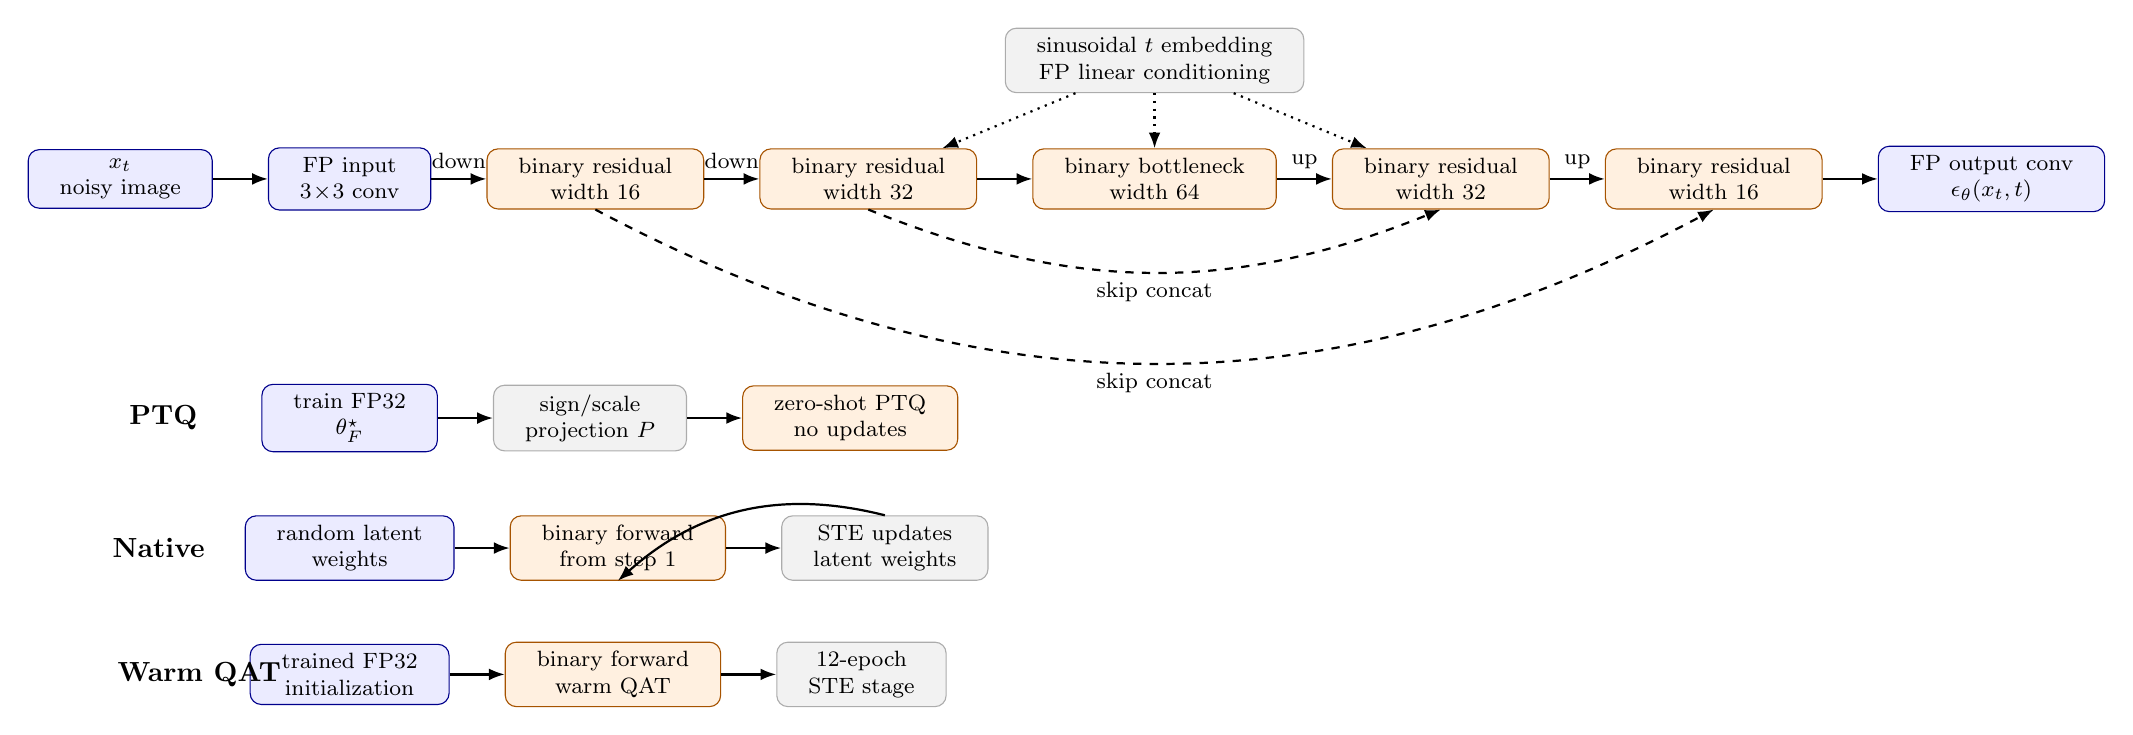
\begin{tikzpicture}[
  font=\footnotesize,
  node distance=5mm and 7mm,
  box/.style={draw,rounded corners,minimum height=7mm,align=center,inner xsep=4mm},
  fp/.style={box,fill=blue!8,draw=blue!55!black},
  bin/.style={box,fill=orange!12,draw=orange!65!black},
  op/.style={box,fill=gray!10,draw=gray!65},
  arrow/.style={-{Latex[length=2mm]},thick}
]
\node[fp] (xt) {$x_t$\\noisy image};
\node[fp,right=of xt] (in) {FP input\\$3\!\times\!3$ conv};
\node[bin,right=of in] (e1) {binary residual\\width 16};
\node[bin,right=of e1] (e2) {binary residual\\width 32};
\node[bin,right=of e2] (mid) {binary bottleneck\\width 64};
\node[bin,right=of mid] (d2) {binary residual\\width 32};
\node[bin,right=of d2] (d1) {binary residual\\width 16};
\node[fp,right=of d1] (out) {FP output conv\\$\epsilon_\theta(x_t,t)$};
\draw[arrow] (xt)--(in);
\draw[arrow] (in)--node[above]{down}(e1);
\draw[arrow] (e1)--node[above]{down}(e2);
\draw[arrow] (e2)--(mid);
\draw[arrow] (mid)--node[above]{up}(d2);
\draw[arrow] (d2)--node[above]{up}(d1);
\draw[arrow] (d1)--(out);
\draw[arrow,dashed] (e1.south) to[bend right=28] node[below]{skip concat} (d1.south);
\draw[arrow,dashed] (e2.south) to[bend right=22] node[below]{skip concat} (d2.south);
\node[op,above=7mm of mid] (time) {sinusoidal $t$ embedding\\FP linear conditioning};
\draw[arrow,dotted] (time) -- (e2);
\draw[arrow,dotted] (time) -- (mid);
\draw[arrow,dotted] (time) -- (d2);

\node[fp,below=22mm of in] (ptq1) {train FP32\\$\theta_F^\star$};
\node[op,right=of ptq1] (ptq2) {sign/scale\\projection $P$};
\node[bin,right=of ptq2] (ptq3) {zero-shot PTQ\\no updates};
\draw[arrow] (ptq1)--(ptq2); \draw[arrow] (ptq2)--(ptq3);

\node[fp,below=8mm of ptq1] (nat1) {random latent\\weights};
\node[bin,right=of nat1] (nat2) {binary forward\\from step 1};
\node[op,right=of nat2] (nat3) {STE updates\\latent weights};
\draw[arrow] (nat1)--(nat2); \draw[arrow] (nat2)--(nat3);
\draw[arrow] (nat3.north) to[bend right=28] (nat2.south);

\node[fp,below=8mm of nat1] (qat1) {trained FP32\\initialization};
\node[bin,right=of qat1] (qat2) {binary forward\\warm QAT};
\node[op,right=of qat2] (qat3) {12-epoch\\STE stage};
\draw[arrow] (qat1)--(qat2); \draw[arrow] (qat2)--(qat3);

\node[anchor=west,font=\bfseries] at ($(ptq1.west)+(-18mm,0)$) {PTQ};
\node[anchor=west,font=\bfseries] at ($(nat1.west)+(-18mm,0)$) {Native};
\node[anchor=west,font=\bfseries] at ($(qat1.west)+(-18mm,0)$) {Warm QAT};
\end{tikzpicture}
}
\caption{Top: compact residual U-Net used in every condition. Binary-marked
convolutions use W1A32 unless the W1A1 core is selected; normalization,
conditioning, scales, residual additions, and boundaries remain FP32. Bottom:
the controlled intervention changes the optimization path, not the topology.}
\label{fig:architecture}
\end{figure*}

\section{Controlled MNIST Experiment}

\subsection{Denoiser and binary forward}

For clean image $x_0$, noise $\epsilon$, and timestep $t$, every condition
minimizes the DDPM noise-prediction objective\cite{ho2020ddpm}:
\begin{equation}
\mathbb E_{x_0,t,\epsilon}\left\|\epsilon-\epsilon_\theta
\left(\sqrt{\bar\alpha_t}x_0+\sqrt{1-\bar\alpha_t}\epsilon,t\right)\right\|_2^2.
\end{equation}
The denoiser in Fig.~\ref{fig:architecture} is a residual U-Net
\cite{ronneberger2015unet} with base width 16, widths $[16,32,64]$, two
downsampling stages, two skip concatenations, GroupNorm, and sinusoidal time
embeddings\cite{vaswani2017attention}. It has 218,993 trainable parameters.

For output filter $W_o$, the primary uncentered binary projection is
\begin{equation}
\widehat W_o=\alpha_o\operatorname{sign}(W_o),\qquad
\alpha_o=\operatorname{mean}(|W_o|).
\end{equation}
Latent FP32 parameters receive identity-STE gradients\cite{bengio2013ste}. The
centered ablation subtracts the filter mean before sign and scale. The W1A1 core
additionally signs block activations with a clipped-identity backward pass.
Input/output convolutions, normalization, time conditioning, biases, scales,
accumulation, and residual additions remain FP32; ``W1A1 core'' therefore does
not mean an end-to-end binary appliance.

\subsection{Conditions and optimization}

FP32 and native conditions train from random initialization for 12 epochs. PTQ
loads the corresponding completed FP32 checkpoint, changes the forward
projection, and performs no optimization. Warm QAT loads that checkpoint and
adds a full 12-epoch binary-forward stage, for 24 total epochs. Native W1A32
crosses centered/uncentered projection with pre-/post-activation residual
ordering\cite{he2016preact}; the headline matched comparison is uncentered and
pre-activation.

We use the canonical 60,000/10,000 MNIST split\cite{lecun1998mnist}, scale
images to $[-1,1]$, and train with AdamW\cite{loshchilov2019adamw}, learning rate
$2\times10^{-4}$, weight decay $10^{-4}$, cosine decay, gradient clipping at 1,
batch size 256, and training seeds $\{0,1,2\}$. Sampling uses all 1,000 ancestral
DDPM steps. Each reported distribution contains 2,000 samples from a fixed
sampling seed independent of the training seed.

\subsection{Evaluation and controls}

An independently initialized MNIST classifier, trained only on the real training
split, reaches 98.03\% test accuracy and 1.44\% ten-bin expected calibration
error. Its penultimate features define domain-feature Fr\'echet distance
(\dfid)\cite{heusel2017fid}, unbiased polynomial-kernel distance
(\dkid)\cite{binkowski2018kid}, and $k=5$ density and coverage
\cite{naeem2020density}. We also report Jensen--Shannon divergence of predicted
class priors. These domain-specific values are not comparable to ImageNet FID.

A disjoint real--real split gives \dfid{} 0.076, density 0.969, and coverage
0.971. Clamped Gaussian noise gives \dfid{} 2278.24 and zero density/coverage.
Although that noise receives mean peak classifier confidence 1.000, confidence
is not used as a quality metric.

\section{Results}

\begin{table*}[t]
\centering
\caption{MNIST metrics, mean $\pm$ sample standard deviation over three training
seeds. Each seed contributes 2,000 samples from the same ancestral sampler.
Bold marks the best non-FP condition, not parity with FP32.}
\label{tab:results}
\small
\begin{tabular}{lrrrrr}
\toprule
Condition & \dfid{} $\downarrow$ & \dkid{} $\downarrow$ & Density $\uparrow$ & Coverage $\uparrow$ & Class JS $\downarrow$ \\
\midrule
FP32 & $3.15\pm0.38$ & $0.056\pm0.013$ & $0.284\pm0.014$ & $0.195\pm0.017$ & $0.033\pm0.009$ \\
Native W1A32, uncentered/pre & $\mathbf{46.33\pm17.24}$ & $\mathbf{1.286\pm0.816}$ & $\mathbf{0.022\pm0.005}$ & $\mathbf{0.033\pm0.010}$ & $\mathbf{0.295\pm0.020}$ \\
Warm QAT W1A32, centered/pre & $66.45\pm28.49$ & $4.945\pm3.686$ & $0.019\pm0.004$ & $0.032\pm0.004$ & $0.320\pm0.059$ \\
Native W1A1 core & $204.55\pm69.77$ & $41.03\pm25.01$ & $0.005\pm0.002$ & $0.009\pm0.004$ & $0.339\pm0.027$ \\
PTQ W1A32, uncentered/pre & $1314.20\pm314.96$ & $2467.50\pm1549.51$ & $0$ & $0$ & $0.531\pm0.002$ \\
\bottomrule
\end{tabular}
\end{table*}

\paragraph{Native optimization mitigates projection collapse.}
Table~\ref{tab:results} gives the main comparison. Native W1A32 has 28.4-fold
lower mean \dfid{} than its matched PTQ configuration and nonzero density and
coverage. This is an empirical witness that a binary-forward optimization path
can reach a substantially better model than sign-projecting the FP32 endpoint.
It does not show that all binary training succeeds: the standard deviation is
large and every reported distribution metric remains worse than FP32.

\paragraph{Warm QAT also recovers.}
Warm QAT obtains \dfid{} $66.45\pm28.49$. Its centered configuration is not a
strictly matched comparison to the best uncentered native row, but its recovery
from PTQ demonstrates that FP initialization is not intrinsically harmful once
the projected model is optimized. Native training is superior to zero-shot PTQ,
not necessarily to every warm-start or teacher-dependent procedure.

\paragraph{W1A1 remains difficult.}
The W1A1 core improves over zero-shot W1A32 PTQ in \dfid{} but has density 0.005
and coverage 0.009. Our experiment therefore does not refute BiDM's observation
that simultaneous weight and activation binarization is difficult. It instead
isolates a weaker but useful statement about one-bit weights with FP32
activations.

\begin{figure}[t]
\centering
\subfloat[FP32]{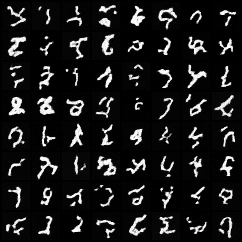
\includegraphics[width=.31\columnwidth]{figures/results/mnist-fp.png}}\hfill
\subfloat[Native W1A32]{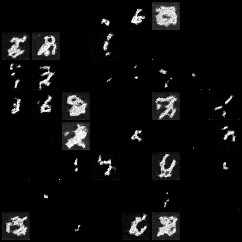
\includegraphics[width=.31\columnwidth]{figures/results/mnist-native-w1a32.png}}\hfill
\subfloat[PTQ W1A32]{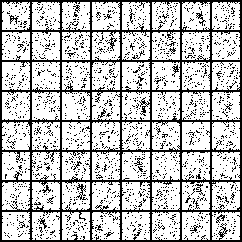
\includegraphics[width=.31\columnwidth]{figures/results/mnist-ptq-w1a32.png}}
\caption{Fixed-seed samples. Native binary-weight training retains digit-like
structure but remains visibly below FP32; zero-shot PTQ collapses.}
\label{fig:samples}
\end{figure}

\begin{table}[t]
\centering
\caption{Native W1A32 architectural ablation (mean \dfid{}; lower is better).}
\label{tab:ablation}
\small
\begin{tabular}{lrr}
\toprule
Residual order & Uncentered & Centered \\
\midrule
Pre-activation & $46.33$ & $99.50$ \\
Post-activation & $84.26$ & $82.46$ \\
\bottomrule
\end{tabular}
\end{table}

\paragraph{Architecture does not yield a universal rule.}
Table~\ref{tab:ablation} shows an interaction: pre-activation helps only without
centering. Centering also raises measured latent-to-projected angular error from
$33.29^\circ$ to $34.05^\circ$ in the pre-activation pair. These results reject
our preliminary centering explanation and do not support a universal claim that
either centering or residual ordering prevents collapse.

\section{Scope, Limitations, and Reproducibility}

This is an MNIST existence result for a small unconditional model. Three seeds
expose high variance but are insufficient for fine-grained significance claims;
2,000 samples per seed make absolute metric estimates noisier than common
50,000-sample evaluations. A separate compact CIFAR-10 attempt is intentionally
excluded from the evidence because its FP32 control also failed, so it could not
adjudicate binary versus floating-point quality on natural images. No theorem
here establishes STE convergence, score approximation, or scaling behavior.

Binary convolutions contain 195,328 of 218,993 parameters. Physical sign packing
plus FP32 scales and remaining tensors gives a 121,316-byte tensor payload versus
875,972 bytes for FP32, a 7.22$\times$ whole-model reduction. This is a storage
measurement: ordinary framework convolutions still execute floating-point
operations, and we claim no latency or energy improvement.

The released pipeline\cite{monodiffuseRepo} records configurations, seeds,
environment versions, source commit, checkpoint SHA-256, histories, metrics,
controls, and packed exports. Exact entry points are under
\path{experiments/v1_binary_study}; the reported artifacts are under
\path{artifacts/v1_binary_study/mnist}. Tests cover parameter compatibility,
forward shapes, diffusion schedules, metric controls, and physical packing.

\section{Conclusion}

Zero-shot projection answers whether one particular FP32 endpoint survives
binarization; it does not answer whether binary-forward optimization can find a
better binary-weight solution. In a controlled MNIST diffusion model, native
W1A32 training reduces domain-feature distance by 28.4-fold relative to matched
PTQ, while warm QAT also recovers substantially. The result is meaningful but
bounded: FP32 remains much better, W1A1 remains weak, and natural-image transfer
is unresolved. Future binary-diffusion comparisons should distinguish native,
warm-started, distilled, and zero-shot training paths rather than treating PTQ
collapse as the limit of the representation.

\smallskip\noindent\textbf{Code availability.}
Source, checkpoints, packed weights, and evaluation artifacts are available at
\url{https://github.com/elixpo/monodiffuse}.

\IEEEtriggeratref{11}
\bibliographystyle{IEEEtran}
\bibliography{references}
\end{document}
